
\documentclass{article}
\usepackage[english]{babel}
\usepackage[utf8]{inputenc}
\usepackage{amsmath} 
\usepackage{fancyhdr}
\usepackage{lastpage}
\usepackage{enumerate}
\usepackage{lineno}
\usepackage{lmodern}
\usepackage{caption}
\usepackage[T1]{fontenc}
\usepackage{microtype}
\usepackage{systeme}
\usepackage{amsmath,amssymb,amsthm,mathrsfs,latexsym,tikz,url}
\usepackage{epigraph,graphicx}
\usepackage{listings}
\usepackage{listingsutf8}
\usepackage{color}
\usepackage{float}

\DeclareGraphicsExtensions{.png,.pdf}
\definecolor{dkgreen}{rgb}{0,0.6,0}
\definecolor{gray}{rgb}{0.5,0.5,0.5}
\definecolor{mauve}{rgb}{0.58,0,0.82}

\lstset{frame=tb,
  language=Python,
  aboveskip=3mm,
  belowskip=3mm,
  showstringspaces=false,
  columns=flexible,
  basicstyle={\small\ttfamily},
  numbers=none,
  numberstyle=\tiny\color{gray},
  keywordstyle=\color{blue},
  commentstyle=\color{dkgreen},
  stringstyle=\color{mauve},
  breaklines=true,
  breakatwhitespace=true,
  tabsize=4
}


\usepackage{hyperref}
\hypersetup{
	colorlinks=true,
	linkcolor=blue,
	filecolor=magenta,      
	urlcolor=cyan,
}
\urlstyle{same}

\setlength{\parindent}{0.0cm}
\setlength{\parskip}{0.1cm}
\setlength{\voffset}{-1in}

\begin{document}

\title{DD2424: Project \\
%The impact of Fourier, and other, transforms in Deep Learning \\
The mechanisms, powers and limitations of some Data Augmentation techniques}

\author{Anton Stråhle, Jan Alexandersson \& Fredrika Lundahl}
\maketitle 

\section{Introduction}

After being briefly introduced to some data augmentation techniques during the lectures we wanted to explore this topic further. 
To deepen our knowledge about this topic we read \href{https://arxiv.org/pdf/1710.09412.pdf} about the data augmentation technique \textit{mixup} which 
really got our interest because of it's ability to improve performance while being very simple. We therefore wanted to further try out this technique 
in practice and compare it with some other data augmentation teqniques, such as color magnification, rotation and other translations, to see how they can improve 
image classification. To clarify, our project does not aim to obtain the highest possible testing accuracy but rather aim to show the impact of data augmentation 
on the accuracy. 

\section{Data}

In this project we will work with a dataset consisting of images of different species of birds, 
\href{https://www.kaggle.com/gpiosenka/100-bird-species}{Bird Species Dataset}. Each image has the format $224 \times 224 \times 3$ and there are 
a total of $190$ species. The training data consist of $25812$ images, but the data is not balanced, however each species has a least $100$ training images. 
Both the validation set and the test set consist of $5$ images of each species. 
It should also be saif that the around $80\%$ of the images are of male birds and $20\%$ of female 
birds which, by the nature of birds, may look entirely different. 
We will not always work with the full dataset but instead pick subsets of some species. 

\section{Mixup}

Mixup is a data augmentation teqnique which creates virtual training example by combining two images by 

\begin{align*}
 &\tilde{x} = \lambda x_i + (1-\lambda) x_j, \qquad \text{where $x_i$, $x_j$ are input vectors} \\
 &\tilde{y} = \lambda y_i + (1-\lambda) y_j, \qquad \text{where $y_i$, $y_j$ are one-hot endoced labels}
\end{align*}


where $(x_i, y_i)$ and $(x_j, y_j)$ are two randomly drawn examples from the training data, and $\lambda$ 
is a probability, that is $\lambda \in [0,1]$. Usually, $\lambda$ is randomly drawn from a Beta$(\alpha, \alpha)$ 
distribution, for each pair of images which are to be combined. This distribution seems like a 
reasonable chioce since it has the right support and the Beta-distribution is the most natural distribution to
consider when working with probabilities. The Beta$(\alpha, \alpha)$-distribution is also symmetric around $0.5$, which may be 
a desireable property, however this should not matter since we combine our randomly drawn examples with weights $\lambda$ and $1-\lambda$ and 
it would not matter if, for example $\lambda = 0.2$ or $\lambda = 0.8$ since it would yield the same two weights, but in different order, but 
since our examples are randomly drawn the order of the weight should not have an impact. 

When reading about mixup, the use of the Beta-distribution is usually taken for granted, however, there are many other distribution which 
could be considered since the only requirement is that the distribution satisfy $\lambda \in [0,1]$. We will therfore not only consider the 
Beta-distribution. 

WRITE ABOUT OTHER DISTRIBUTION(S) (logit-normal)

We will also consider only performing mixup on the input vectors of the training images but letting $\tilde{y}$ keep the label of the exemple 
with the highest weight. That is,

\begin{align*}
 \tilde{y} = I_{\{ \lambda \leq 0.5 \}} y_i + (1-I_{\{ \lambda \leq 0.5 \}}) y_j, 
\end{align*}

where $I_{\{ \lambda \leq 0.5 \}} = 1$ if $\lambda \leq 0.5$ and $0$ otherwise.



\begin{figure}[!htb]
\minipage{0.32\textwidth}
  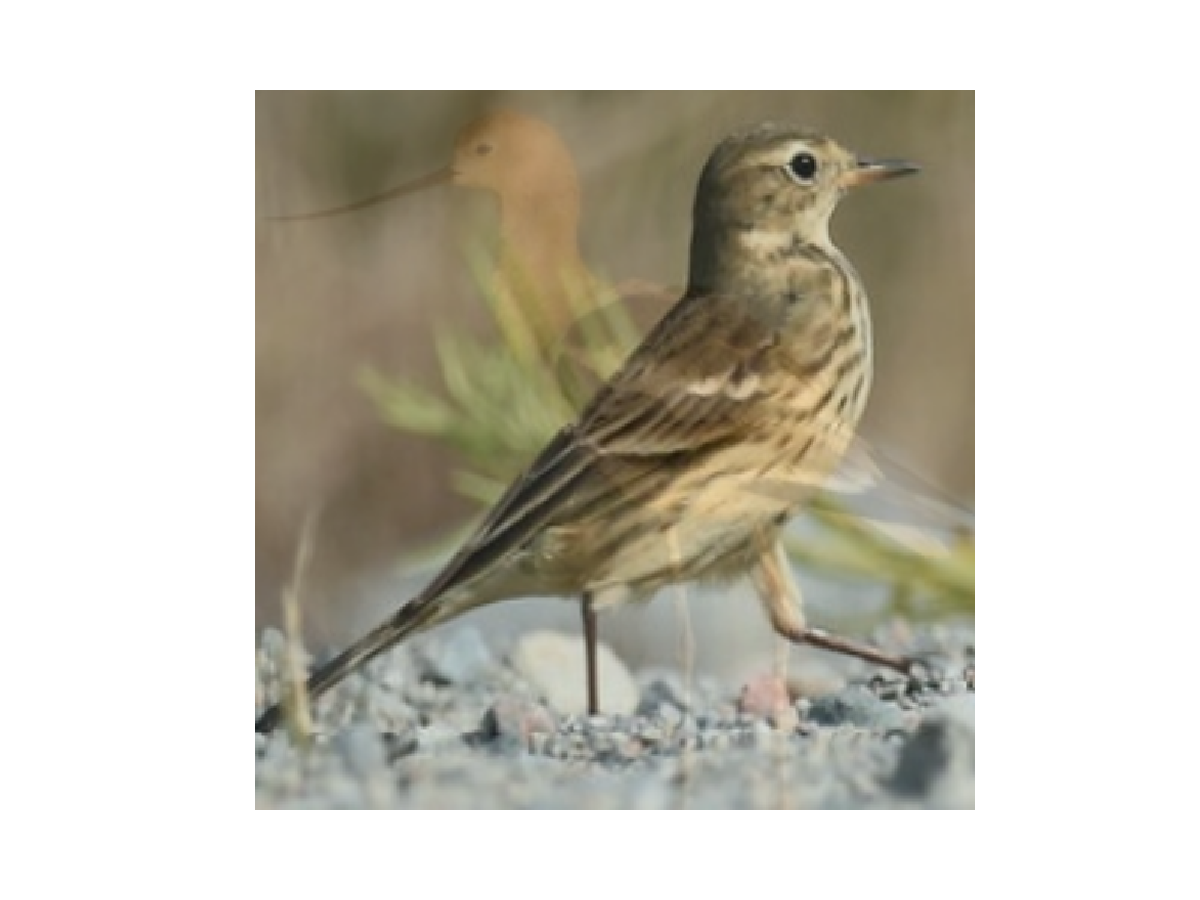
\includegraphics[trim=3cm 2cm 3cm 3cm, width=\linewidth]{mixup1.pdf}
\endminipage\hfill
\minipage{0.32\textwidth}
  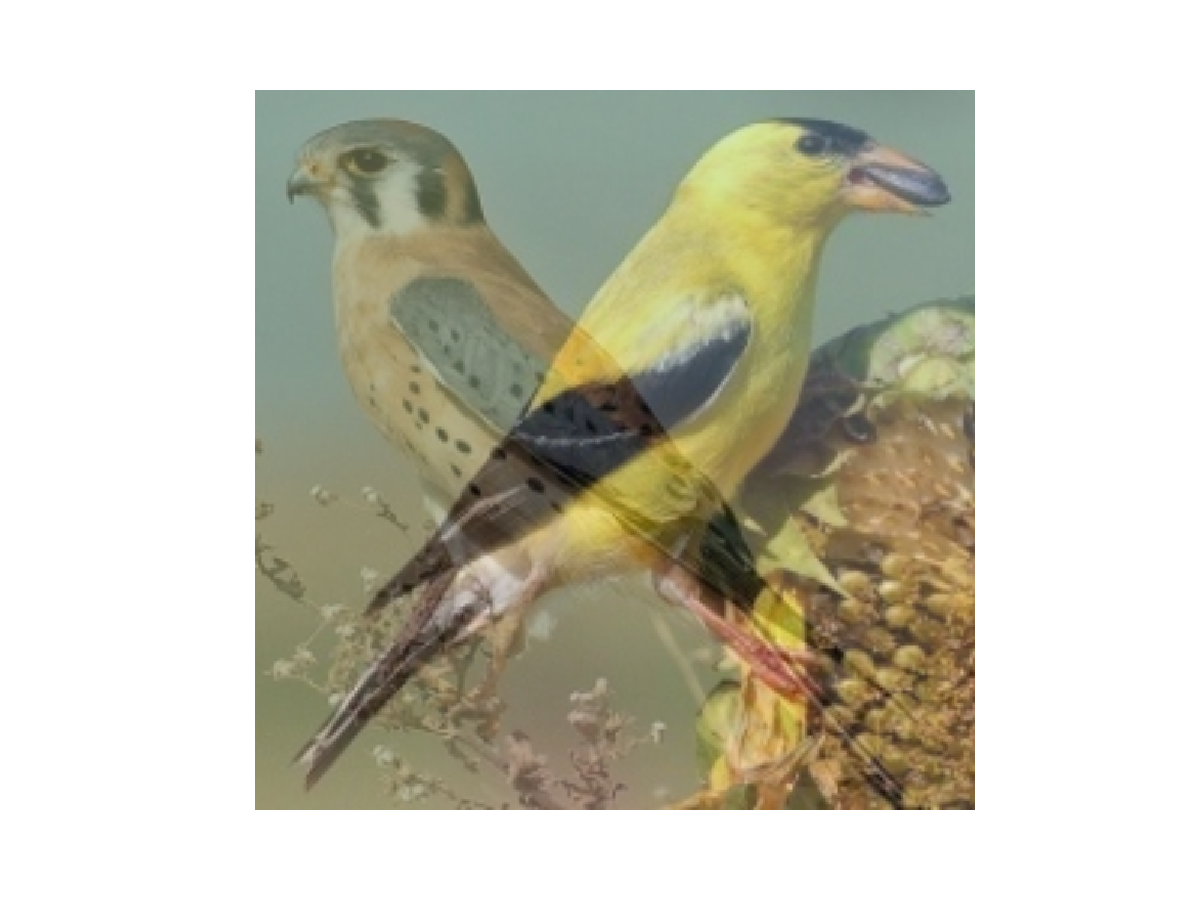
\includegraphics[trim=3cm 2cm 3cm 3cm, width=\linewidth]{mixup2.pdf}
\endminipage\hfill
\minipage{0.32\textwidth}%
  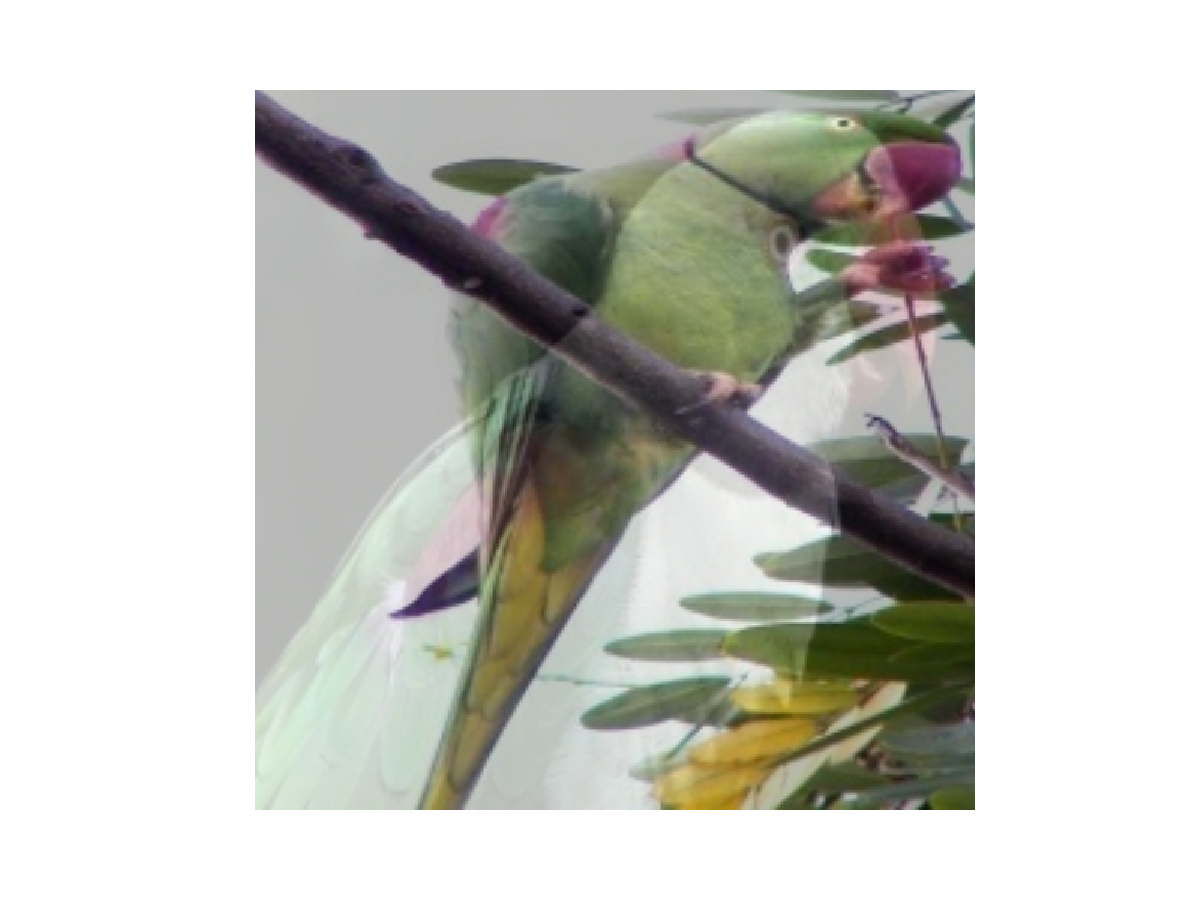
\includegraphics[trim=3cm 2cm 3cm 3cm, width=\linewidth]{mixup3.pdf}
\endminipage
\caption{Three examples of mixup on images of different birds.}
\end{figure}

\section{Experiments}




\end{document}
